\chapter{Resultados numéricos}\label{Cap:ResultadosNumericos}
\linenumbers
En este capítulo se presentan los resultados numéricos obtenidos durante el desarrollo de este trabajo. En primera instancia, se valida la implementación corrotacional detallada en el Capítulo \ref{Cap:Preliminares}, para luego aplicarse a modelos específicos de conductores. Todas las simulaciones fueron realizadas utilizando un computador portátil con un procesador i7 6700HQ y una memoria ram de 8 Gb. La formulación se implementó en el software de código abierto \href{https://github.com/ONSAS/ONSAS.m/}{ONSAS} el cual se ejecutó en GNU-Octave presentado por \cite{eaton2007gnu} y visualizándose los resultados haciendo uso de la herramienta Paraview publicada en \citep{ahrens2014image}. Vale notar que el hilo conductual de este capítulo fue ideado con un aumento progresivo de complejidad. En el ejemplo de la Sección \ref{Sec:RN:FotiCable} valida las funciones implementadas, luego en el ejemplo de la Sección \ref{Sec:RN:FotiCable} se obtienen resultados para un primer modelo de cables y finalmente en el ejemplo de la Sección \ref{Sec:RN:TransmissionSystem} se aplica la implementación validada a la simulación del comportamiento de sistemas de transmisión eléctrica sometidas a la acción de CC.


\section{Viga en voladizo con ángulo recto}\label{Sec:RN:RightAngle}
Este ejemplo fue publicado por primera vez en \citep{simo1988dynamics} y es usualmente considerado en la literatura para validar implementaciones de elementos de viga tridimensionales aplicadas a estructuras no lineales (\citep{albino2018co} \citep{Le2014}). El mismo consta de dos barras idénticas en ángulo recto formando una forma de L. Cada miembro que la integra, mide un largo $L=10$ m tal y como se ilustra en la Figura \ref{fig:RN:RA:esquemas}.

\begingroup
\centering
\begin{figure}[htbp]
	\centering
	\subfigure[Vista frontal ]{	\def\svgwidth{60mm}
		\input{./imagenes/ResultadosNumericos/RightAngeCantilever/Ilustracion2Dxy.pdf_tex}}\label{fig:RN:RA:Ilusxy}
	\subfigure[Vista lateral ]{	\def\svgwidth{41mm}
	\input{./imagenes/ResultadosNumericos/RightAngeCantilever/Ilustracion2Dyz.pdf_tex}}\label{fig:RN:RA:Ilusyz}
	\caption{Disposición geométrica de la estructura.} 	\label{fig:RN:RA:esquemas}
\end{figure}
\endgroup

Las rigideces de torsión, flexión y directa del ejemplo se seleccionaron de manera sintética por el autor original. Estos valores artificiales, garantizan movimientos de gran amplitud y para esto deben cumplir determinadas igualdades a continuación:

\begin{eqnarray}
	\label{eq:RN:RA:Propiedades1}
	GA &= EA& =10^6\\
	\label{eq:RN:RA:Propiedades2}
	GJ &= EI& =10^3.
\end{eqnarray}

Dado esto la elección de dichas magnitudes se obtiene resolviendo el sistema compatible indeterminado de Las Ecuaciones \eqref{eq:RN:RA:Propiedades1} y \eqref{eq:RN:RA:Propiedades2}. Para este trabajo el autor escogió los siguientes valores: $ E=G=10^6$ $A=1 $  $I=J=10^{-3}$ y $\nu=0.3$. Se hace notar que el carácter arbitrario de los parámetros implica que sus unidades carezcan de sentido. 


La estructura se encuentra empotrada en su base imponiendo desplazamientos y ángulos nulos en el nodo C. Este apoyo ejerce reacciones que permiten aplicar una fuerza en el sentido del eje $z$ tal y como se muestra en la Figura \ref{fig:RN:RA:esquemas}. Este forzante flecta y torsiona al sistema en un plano saliente al $xy$, produciendo oscilaciones de gran amplitud. En la expresión anterior el adjetivo gran, hace alusión a que los movimientos desarrollados durante el movimiento, los cuales son del mismo orden de magnitud que las dimensiones de la estructura. Estos desplazamientos significativos, están ligados al perfil brusco de aplicación de la carga. Esta fuerza crece linealmente en los dos segundos iniciales, crece hasta un valor máximo de $50$ N en el primer segundo de simulación y luego decrece hasta cero. Imponiendo en el perfil un impacto severo y gradual en un corto intervalo de tiempo como se muestra en la figura a continuación: 

\begin{figure}[htbp]
	\centering
	\def\svgwidth{80mm}
	\input{./imagenes/ResultadosNumericos/RightAngeCantilever/FuerzaZ.pdf_tex}
	\caption{Perfil de fuerza transversal en el nodo A.}
	\label{fig:RN:RA:Force}
\end{figure}

El objetivo principal del ejemplo es validar los códigos incorporados al software \href{https://github.com/ONSAS/ONSAS.m/}{ONSAS}, por ende, tanto el método de resolución, como los parámetros, se ajustaron idénticos a los explicitados en el artículo \citep{Le2014}, comparando así resultados semejantes. Consecuentemente se seleccionó un valor característico $\alpha=-0.05$ y un valor de parada en desplazamientos de $10^{-7}$ m. Se fraccionaron 20 $s$ de simulación en intervalos de $\Delta T=0.25$ s y se discretizó la geometría con 10 elementos por barra.

Para ilustrar al lector en la cinemática del movimiento, se graficaron las deformadas para diferentes instantes de tiempo: $t_1=4$ s, $t_2=11$ s y $t_3=19$ s. En la Figura \ref{fig:RN:RA:Deformadas} se observan las oscilaciones flexionales para distintos planos $yx$ e $yz$. Estos movimientos son originados por diferentes razones, en la barra $\text{CA}$ se asocia al forzante $F_z$ mientras que en el miembro $\text{AB}$ son generados por los vínculos cinemáticos e inerciales debido a su unión rígida con el resto de la estructura.

\begin{figure}[htbp]
	\centering
	\def\svgwidth{120mm}
	\input{./imagenes/ResultadosNumericos/RightAngeCantilever/Deformadas.pdf_tex}
	\caption{Estructura deformada en los instantes $4$ s, $11$ s y $21$ s.}
	\label{fig:RN:RA:Deformadas}
\end{figure}  

Con el objetivo de comparar los resultados del artículo de referencia se graficaron ciertos desplazamientos del nodo A. Estos son: el desplazamiento lineal vertical (según el eje $y$) y el transversal (según $z$). Los resultados extraídos del modelo se muestran en las Figuras \ref{fig:RN:RA:DispsA} en función de la variable temporal. En estas se constata efectivamente la significativa magnitud de los desplazamientos en comparación con las dimensiones de la estructura. En particular, la Figura \ref{fig:RN:RA:DispzA} denota oscilaciones que alcanzan varios metros en menos de 30 segundos, esto muestra el carácter exigente en términos dinámicos del ejemplo. Con respecto a este movimiento no armónico  de vaivén en el eje $z$, se puede notar la presencia del amortiguamiento artificial introducido por el método de resolución numérica, ya que las amplitudes prestan una tendencia atenuante con el tiempo.  

\begingroup
\centering
\begin{figure}[htbp]
	\centering
	\subfigure[Desplazamiento vertical según $y$ ]{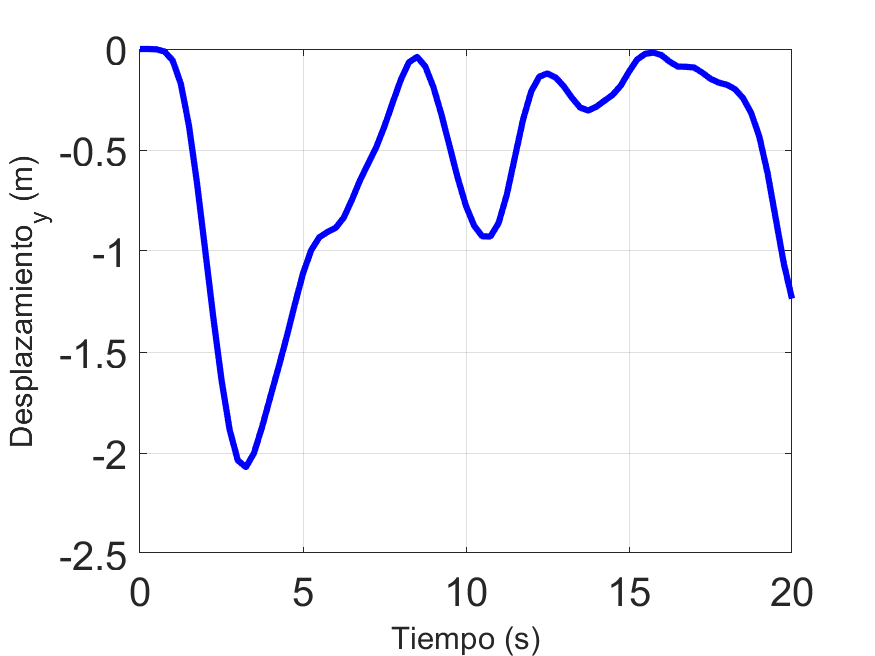
\includegraphics[width=0.48\textwidth]{./imagenes/ResultadosNumericos/RightAngeCantilever/RA_Dispy_NodeA.png}\label{fig:RN:RA:DispyA}}
	\subfigure[Desplazamiento transversal según $z$ ] {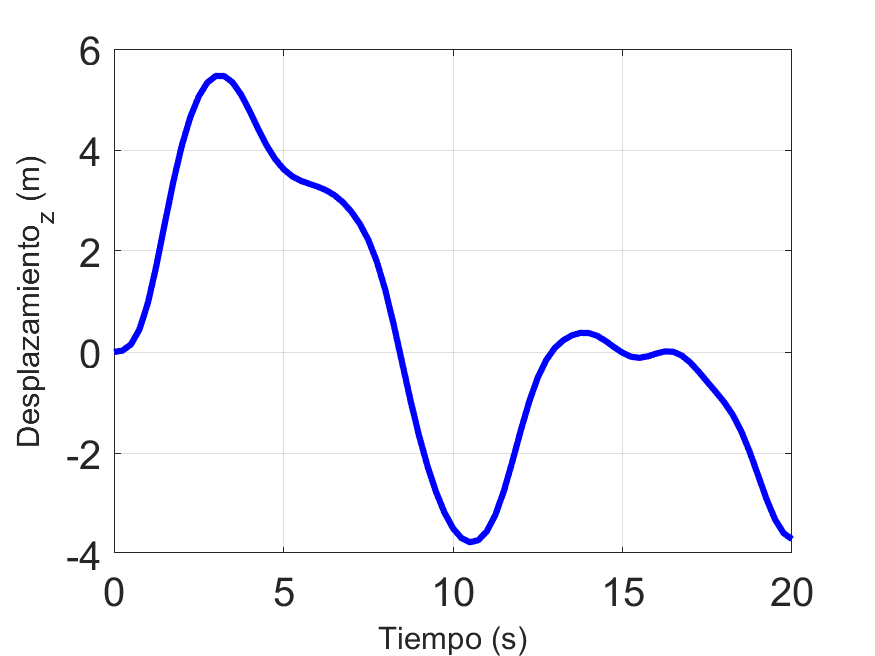
\includegraphics[width=0.48\textwidth]{./imagenes/ResultadosNumericos/RightAngeCantilever/RA_Dispz_NodeA.png}\label{fig:RN:RA:DispzA}}
	\caption{Desplazamientos de control del nodo A.} \label{fig:RN:RA:DispsA}
\end{figure}
\endgroup

Por otra parte al analizar en la Figura \ref{fig:RN:RA:DispyA} se observa que los desplazamientos en $y$, son menores a cero para todo instante, esto se vincula al sentido de la fuerza aplicada. Al observar la estructura desde un plano $yz$ con el versor $x$ saliente, el movimiento del nodo $A$ es análogo al de una viga empotrada con una fuerza cortante en su extremo. De esta manera, el desplazamiento de A es siempre en el sentido de $-y$, lo que se refleja en La Figura \ref{fig:RN:RA:DispyA} y condice con la respuesta esperada. Contrastando los resultados de la implementación con los presentados en la bibliografía de \cite{Le2014}, se observan similares valores de máximos y mínimos alcanzados durante el movimiento respecto a las Figuras \ref{fig:RN:RA:DispsA} y \ref{fig:RN:RA:DispsB}. También así los valles y las crestas de la curvas se suceden en tiempos muy próximos. Congruentemente, es posible afirmar que las funciones implementadas en \href{https://github.com/ONSAS/ONSAS/}{ONSAS} reproducen correctamente el ejemplo y es capaz de capturar movimientos de flexo-torsión para grandes desplazamientos y rotaciones cabalmente. 


\begingroup
\centering
\begin{figure}[htbp]
	\centering
	\subfigure[Desplazamiento vertical según $y$ ]{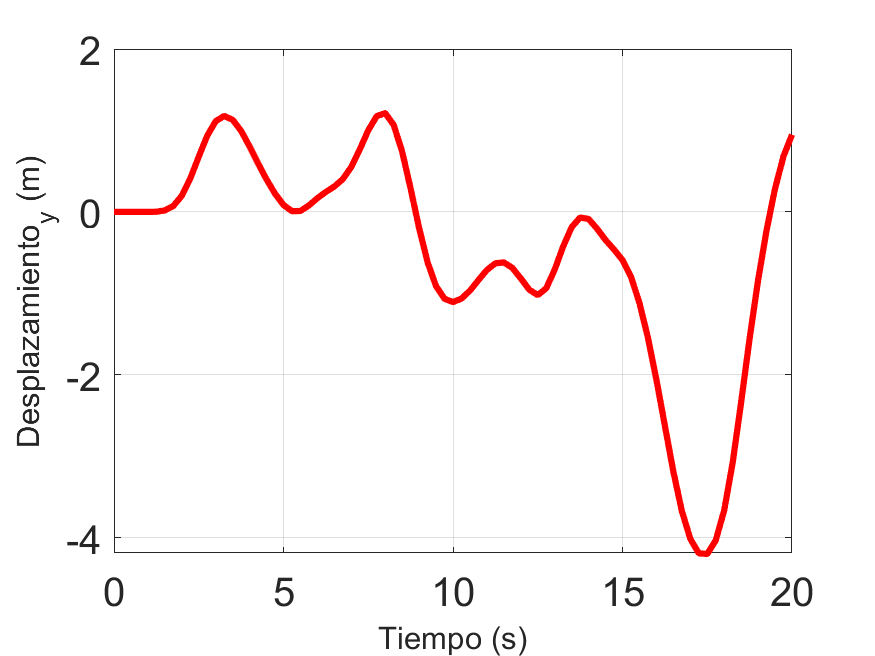
\includegraphics[width=0.48\textwidth]{./imagenes/ResultadosNumericos/RightAngeCantilever/RA_Dispy_NodeB.png}\label{fig:RN:RA:DispyB}}
	\subfigure[Desplazamiento transversal según $z$ ] {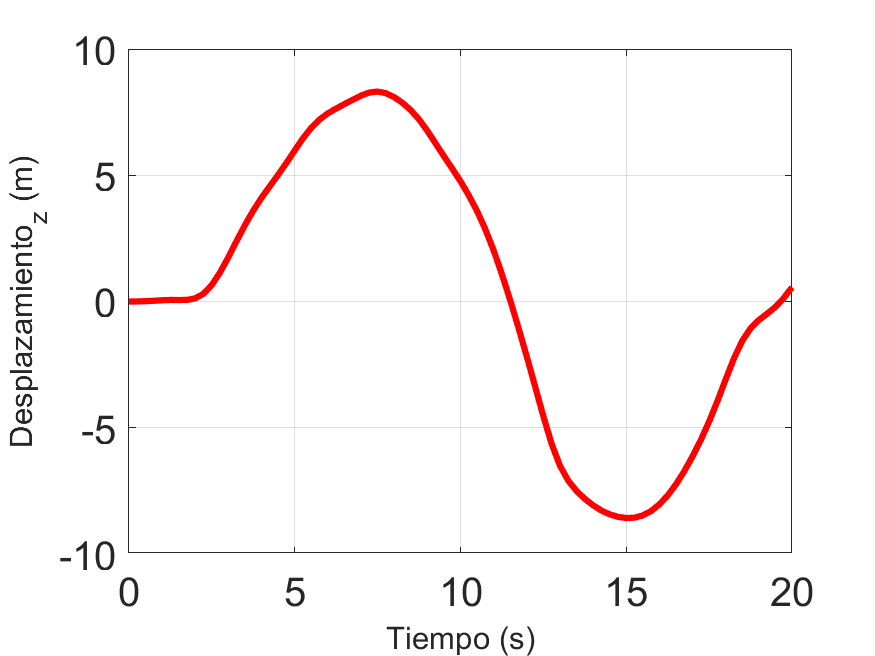
\includegraphics[width=0.48\textwidth]{./imagenes/ResultadosNumericos/RightAngeCantilever/RA_Dispz_NodeB.png}\label{fig:RN:RA:DispzB}}
	\caption{Desplazamientos de control del nodo B.} \label{fig:RN:RA:DispsB}
\end{figure}
\endgroup

Resulta oportuno analizar los movimientos en el nodo B. En la Figura \ref{fig:RN:RA:DispzB} se muestra una oscilación de 16 metros de amplitud aproximadamente, y una forma que se asemeja a una sinusoide. Esto podría vincularse al modo flector en el plano $xz$ de la barra A-B excitado por la fuerza externa en la dirección $z$. Una vez retirada la carga se manifiestan los modos torsionales de AC superpuestos con los flexionales de A-B C-B incidiendo en el movimiento. El autor del trabajo \textcite{Le2014} publicó el desplazamiento en $z$ de B y los resultados de este trabajo ajustan con exactitud a dicha curva. 

Habiéndose ahondado en las variables cinemáticas, resta por analizar las magnitudes dinámicas. Para esto se colorearon los esfuerzos normales inmanentes a cada elemento en La Figura \ref{fig:RN:RA:Deformadas}. En esta se identifica que el esfuerzo alcanza valores de compresión y tracción en similar magnitud presentando considerables fluctuaciones temporales. En simultaneo, la viga horizontal $\text{A-B}$ desarrolla fuerzas normales en todo su largo. 

%Se suceden tanto positivas como negativas, es oportuno notar que un modelo lineal para pequeños desplazamientos concluiría que los esfuerzos en esa viga serían nulos. Además este modelo lineal arrojaría desplazamientos triviales en $x$ para ambos nodos, induciéndose significativos errores para este tipo de cargas de alto impacto en estructuras de exigua rigidez. 

El modelo implementado desarrolla magnitudes no despreciables de desplazamientos en $x$ tal y como se constata en las Figuras \ref{fig:RN:RA:DispsXAB}. He aquí  la importancia de implementar un modelo considerando no linealidad geométrica, estas consideraciones son esenciales para la aplicación principal de este trabajo.  


\begingroup
\centering
\begin{figure}[htbp]
	\centering
	\subfigure[Desplazamiento según $x$ del nodo B]
	{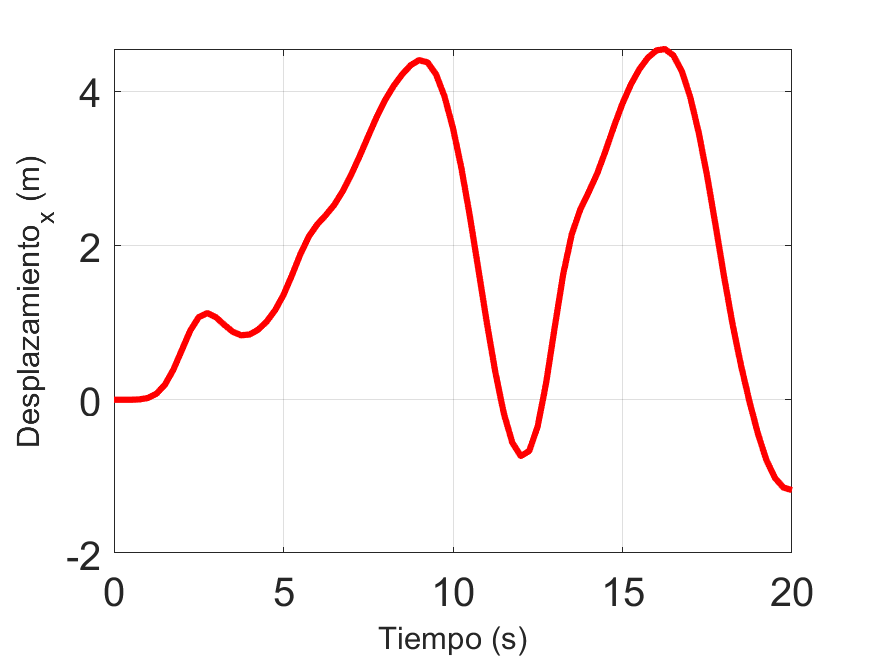
\includegraphics[width=0.48\textwidth]{./imagenes/ResultadosNumericos/RightAngeCantilever/RA_Dispx_NodeB.png}}\label{fig:RN:RA:DispxB}
	\subfigure[Desplazamiento según $x$ del nodo A ] {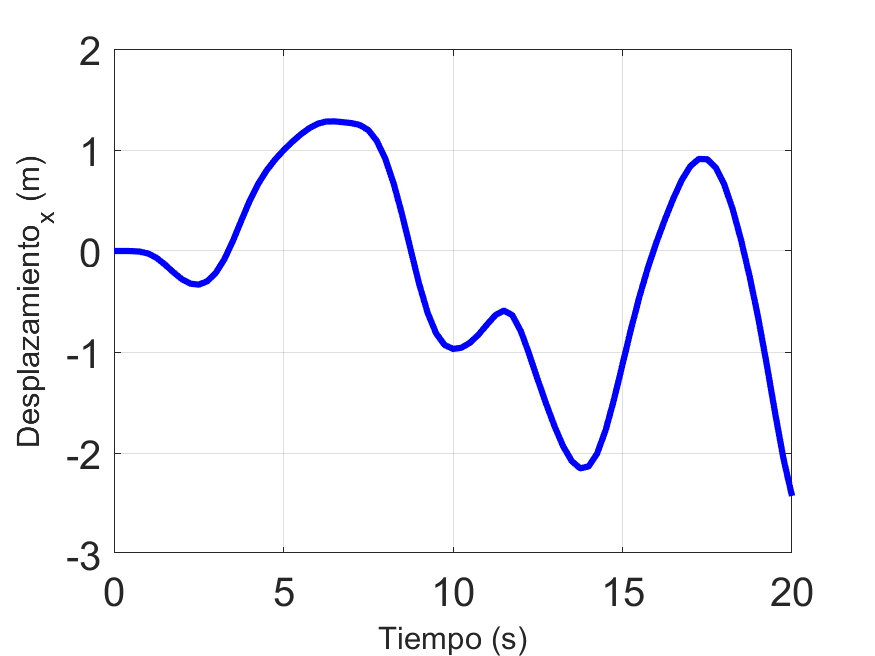
\includegraphics[width=0.48\textwidth]{./imagenes/ResultadosNumericos/RightAngeCantilever/RA_Dispx_NodeA.png}}\label{fig:RN:RA:DispxA}
	\caption{Desplazamientos en x de los nodos A y B} \label{fig:RN:RA:DispsXAB}
\end{figure}
\endgroup

\section{Modelo simplificado de una línea}\label{Sec:RN:FotiCable}
En esta sección se presenta un primer modelo simplificado del enfoque central de esta tesis. El mismo fue contrastado con el trabajo de \cite{foti2018finite} aunque ha sido abordado por destacados investigadores en el pasado, como ser el caso de: \cite{luongo1998non}, \cite{martinelli2001numerical}. El ejemplo consiste en un conductor de transmisión eléctrica reforzado con núcleo de acero sometido a un perfil de viento artificial. 

Con el propósito de aproximarse a la configuración del conductor dispuesto en un sistema de transmisión eléctrica real, se introdujeron al ejemplo dos cadenas aisladoras en posición vertical, de un largo $L_a=3$ m cada una de ellas. Estos elementos no reciben fuerza y no se estudiará el desplazamiento ni esfuerzos en los mismos. Esto se aseguró en las condiciones de borde impuestas, para el modelo se consideró una condición de desplazamiento y ángulo nulo en las tres direcciones en $x$, $z$ e $y$ en los puntos $\text{B}$ y $\text{C}$. Dado esto, las cadenas solo toman un rol ilustrativo gráfico y las restricciones de borde representan correctamente las presentadas por \cite{foti2018finite}, donde los extremos se encuentran sujetados. Habiendo detallado someramente los componentes que integran al ejemplo se presenta un esquema de la geometría a continuación:

\begin{figure}[htbp]
	\centering
	\def\svgwidth{80mm}
	\input{./imagenes/ResultadosNumericos/SimpleCable/EsquemaCable.pdf_tex}
	\caption{Esquema ilustrativo del ejemplo de un conductor simplificado.}
	\label{fig:RN:FotiCable:Ilustracion}
\end{figure}


El vano tiene un largo Lc=$267$ m y para esta simulación no se tendrá en cuenta la tensión previa al momento de la colocación, pero sí la tensión debida a la carga del peso. Por otra parte, el modelo del conductor esta estandarizado bajo la norma europea \citep{IEC60826} y se identifica con la nomenclatura DRAKE ASCR 7/26. Esto hace referencia a la cantidad de cables en el núcleo y en la periferia, respectivamente. El diámetro se calcula entonces como la composición del área de los 26 conductores hechos de aluminio (color gris) y los 7 de acero (color azul). El perfil del conductor se ilustra en la siguiente figura: 

\begin{figure}[htbp]
	\centering
	\def\svgwidth{80mm}
	\input{./imagenes/ResultadosNumericos/SimpleCable/PerfilCable.pdf_tex}
	\caption{Esquema del conductor  ASCR 7/26.}
	\label{fig:RN:FotiCable:Perfil}
\end{figure}
%La raíz de acero forjado del conductor tiene como propósito aportar rigidez mecánica al componente, disminuyendo la deflexión y flexibilidad del conjunto. Esto suele ser ventajoso para largos vanos donde la rigidez del conductor es una variable decisiva. Además, su construcción no afecta significativamente la resistividad eléctrica debido al efecto de reluctancia radial variable. que obliga a la corriente a fluir principalmente en la superficie. 
El material que constituye al cable tiene un módulo de elasticidad $E$, coeficiente de Poissón $\nu$, una densidad $\rho$ y una rigidez flexional y torsional $EI$ y $GJ$, respectivamente. Estas propiedades descritas se obtuvieron de \citep{Foti2016} y se presentan en La Tabla a continuación:

\begin{table}[ht!]
	\begin{center}
		\begin{tabular}{ | m{2cm} | m{2cm} | m{2cm} | m{2cm} |  m{2cm} | }
			\hline $d_c$ (cm) & m (kg/m)& $EA$ (kN)& $EI$ (N.m$^2$)& $GJ$ (N.m$^2$)  \\ \hline
			2.81 & 1.8 & 29700 &2100 &159   \\ \hline
		\end{tabular}
	\end{center}
	\caption{Propiedades mecánicas del conductor DRAKE ASCR 7/26 }
	\label{table:RN:FotiCable:propiedadesCable}
\end{table}

Existen diferencias sustancial respecto al ejemplos originales postulados por \cite{luongo1998non} y \cite{martinelli2001numerical}, en donde se resolvió mediante elementos de barra trinodal y de viga corrotacional, respectivamente. Para ambos trabajos se consideraron efectos de turbulencia generada artificialmente mediante procesos estocásticos, mientras que para este estudio se desprecia las componentes fluctuantes, teniendo en cuenta el mismo flujo medio $W$  en la coordenada axial del conductor. Este perfil es parabólico y alcanza la velocidad media máxima $W_{max}$ en $20$ segundos. Este valor de velocidad se calculó según \citep{IEC60826} considerando un flujo tipo CLA con las propiedades indicadas en la siguiente Tabla considerando a un tipo de terreno sub-urbano o industrial:


\begin{table}[htbp]
	\begin{center}
		\begin{tabular}{ | m{2cm} | m{2cm} | m{2cm} | }
			\hline $k_r$ & $z_0$& $z_{min}$  \\ \hline
			$0.22$ &$0.3$ m & $8$ m     \\ \hline
		\end{tabular}
	\end{center}
	\caption{Parámetros del flujo tipo CLA para $W_{max}$ }
	\label{table:RN:propiedadesFlujo}
\end{table}

La simulación consta de dos etapas, primeramente se aplica la fuerza gravitatoria según el eje $-z$  y luego las fuerzas del viento tal e las direcciones que se muestra en la Figura \ref{fig:RN:FotiCable:Ilustracion}. No se muestran los resultados de esta etapa debido a que carecen de relevancia y en el trabajo de referencia se toma la catenaria como condición inicial. Una vez estabilizada la respuesta del sistema por el amortiguamiento interno, se aplica una fuerza lineal de media positiva según el eje $-z$ desde cero hasta $W_{max}$. Esta forma del perfil podría emular el aumento modulado de presiones en un túnel de viento entre las bocas de entrada y descarga. La forma del perfil se muestra en la siguiente figura:
\begin{figure}[ht!]
	\centering
	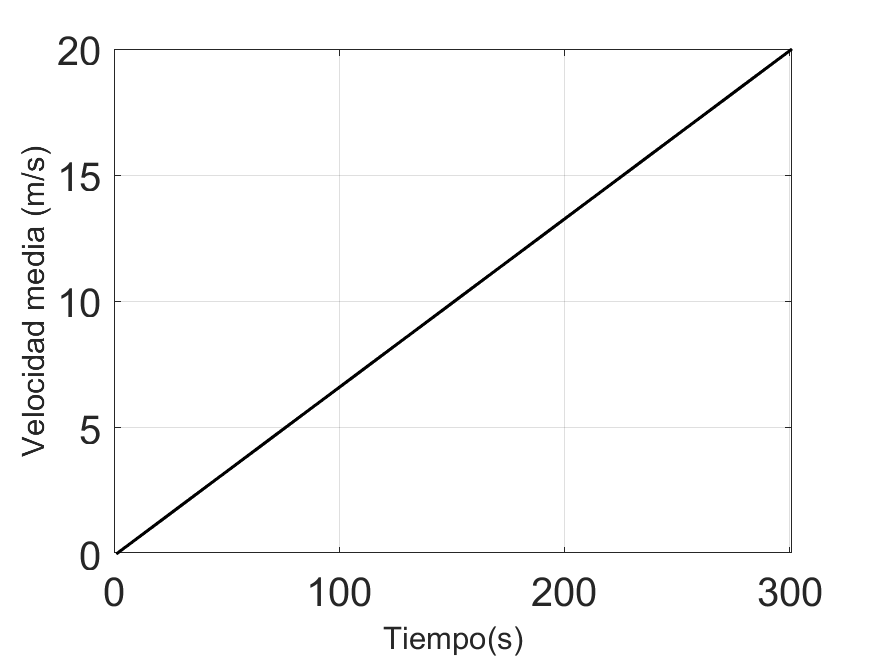
\includegraphics[width=80mm]{./imagenes/ResultadosNumericos/SimpleCable/PerfilVm_TL_Foti.png}
	\caption{Perfil de velocidad progresiva $z$.}
	\label{fig:RN:FotiCable:VelocidadCable}
\end{figure}

Para este estudio no se considerará la fuerza de \textit{lift}. Esta es despreciada por diferentes autores \cite{lee1992nonlinear}, \cite{Foti2016} y \cite{Papailiou1997} principalmente porque la razón de fuerzas en las componentes perpendiculares a los flujos está relacionada con posibles asimetrías tangenciales en el perfil. Para conductores sin formaciones de hielo en su superficie, la circulación del campo de velocidades relativo circundante es próxima a cero, lo que se traduce en una fuerza de \textit{lift}. nula. Esta es la principal diferencia de este caso en comparación por lo propuesto en la literatura por \cite{luongo1984planar} y \cite{foti2018finite} donde los perfiles presentan formaciones de hielo.

Se considera un flujo transversal al eje del cable, con una historia de velocidad media mostrada en la Figura \ref{fig:RN:FotiCable:VelocidadCable}. Los valores de $C_d=1.5$ se extrajeron la referencia de \citep{foti2018finite}. Se aclara que el ángulo de ataque varía durante la trayectoria del cable, no obstante, el coeficiente $C_d$ permanece constate debido a la simetría de revolución del perfil. Se muestran entonces las fuerzas sobre cada nodo del conductor en la figura a continuación:


\begin{figure}[h]
	\centering
	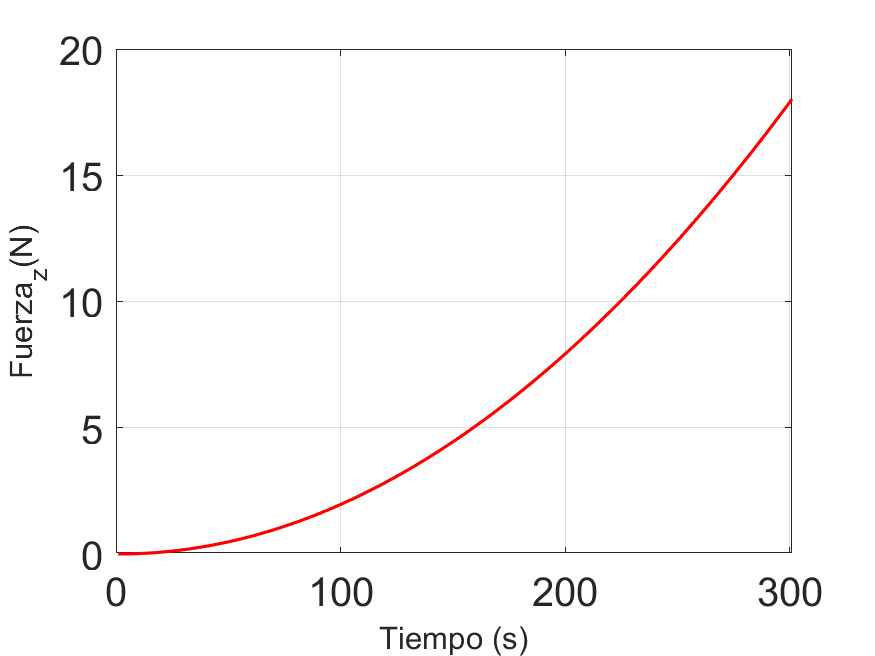
\includegraphics[width=80mm]{./imagenes/ResultadosNumericos/SimpleCable/FuerzaNodalZ_TLFoti.png}
	\caption{Perfil de fuerza nodal según el eje $z$.}
	\label{fig:RN:FotiCable:FuerzaZ}
\end{figure}


%A continuación se exponen los desplazamientos verticales y horizontales del nodo $\text{A}$. En estos se observa un comportamiento inercial y una relación entre el perfil de fuerza y desplazamientos. Esta homología entre los perfiles de ambas magnitudes es explicable mediante un análisis de Fourier del sistema. Haciendo referencia a la función de transferencia que relaciona a ambas variables, la misma produce únicamente en desfasaje en estado estacionario. Como la curva de carga es de manera gradual y no presenta exabruptos en el tiempo, se supone que la respuesta es cuasi-estática. 

Se presentan a continuación los desplazamientos en vertical y transversal del nodo A, respectivamente, situado en el punto medio del vano :

\begingroup
\centering
\begin{figure}[htbp]
	\centering
	\subfigure[Desplazamiento según $z$ del nodo A]
	{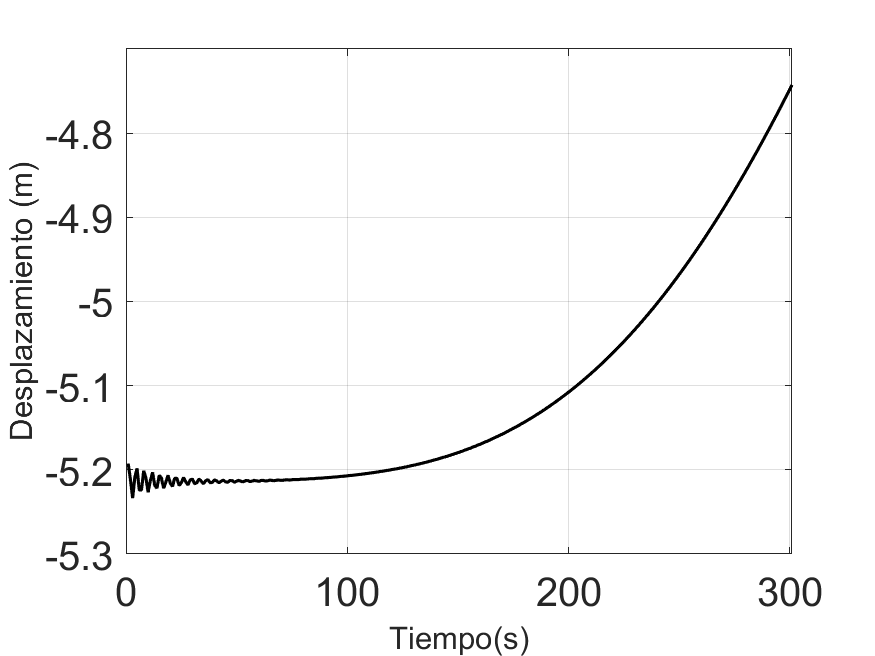
\includegraphics[width=0.48\textwidth]{./imagenes/ResultadosNumericos/SimpleCable/DispZTL_Foti.png}\label{fig:RN:FotiCable:DispZ}}
	\subfigure[Desplazamiento según $y$ del nodo A ] {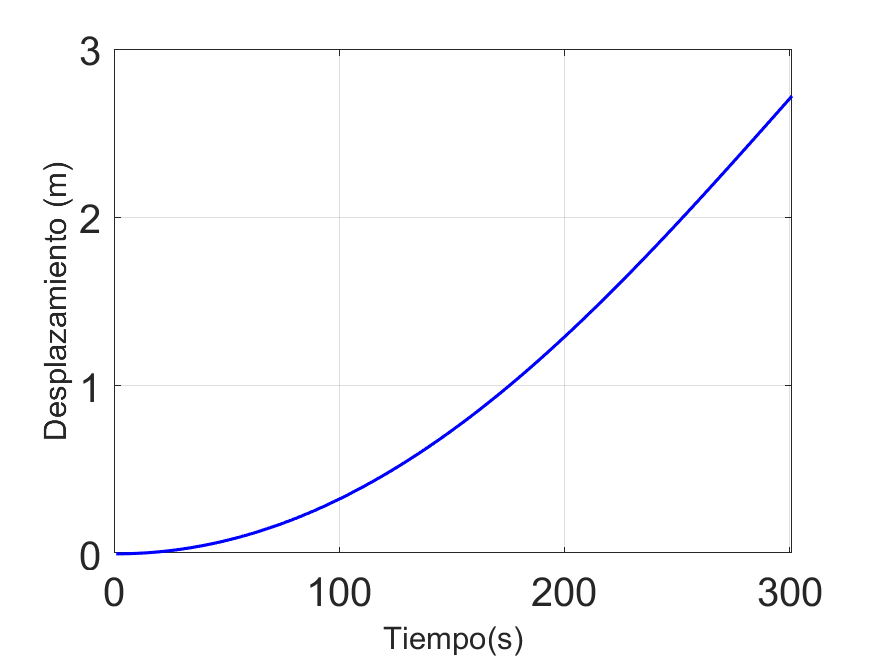
\includegraphics[width=0.48\textwidth]{./imagenes/ResultadosNumericos/SimpleCable/DispYTL_Foti.png}\label{fig:RN:FotiCable:DispY}}
	\caption{Desplazamientos del nodo A.} \label{fig:RN:FotiCable:DispsA}
\end{figure}
\endgroup

Con el objetivo de contrastar los resultados tomando como referencia la literatura fuente (\textcite{foti2018finite}), se capturo el ángulo de balanceo del punto $\text{A}$ para todo tiempo. Esta variable se halla mediante la función tangente que vincula el ángulo respecto da la deformada en el eje $x$ con los desplazamientos en $z$ e $y$. Para ilustrar al lector se realizó el siguiente esquema del ángulo $\Phi$:

\begin{figure}[htbp]
	\centering
	\def\svgwidth{80mm}
	\input{./imagenes/ResultadosNumericos/SimpleCable/AnguloCable.pdf_tex}
	\caption{Esquema ilustrativo del ejemplo de un conductor simplificado.}
	\label{fig:RN:FotiCable:Angulo}
\end{figure}


Se graficaron las trayectorias del ángulo para diferentes valores de velocidad media de viento, generando así una curva carga desplazamiento aerodinámica. Es posible notar que la forma de la Figura \ref{fig:RN:FotiCable:Angulo} describe un perfil semejante al que desarrollan tanto la fuerza, como los desplazamientos en las Figuras \ref{fig:RN:FotiCable:DispsA} y \ref{fig:RN:FotiCable:FuerzaZ}. Esta similitud se fundamenta en que la velocidad es lineal con el tiempo y por tanto, su escala es proporcional a la temporal.
Por otra parte, en comparación con los resultados presentados por \cite{foti2018finite} se observan valores similares de ángulo para las diferentes velocidades. Asimismo, la forma del perfil es idéntica para todo el dominio temporal. Sin embargo, el valor máximo de ángulo alcanzado en este modelo es mayor comparativamente, lo que se puede atribuir al menos a dos factores. En primera instancia la turbulencia introducida en la bibliografía atenúa los desplazamientos debido a que las fluctuaciones axiales en el perfil de viento, se ejercen fuerzas desincronizadas a lo largo del vano mientras que en este modelo las fuerzas se acompasan produciendo mayores amplitudes. El segundo factor se vincula a la presencia del \ y la variación del ángulo de ataque con el ángulo. Como en la referencia \citep{foti2018finite} se toman en cuenta un perfil con formaciones de hielo, y por tanto sin simetría de revolución, las fuerzas generadas afectan de diferente forma al conductor de estudio produciendo resultados discordantes. 


\begin{figure}[htbp]
	\centering
	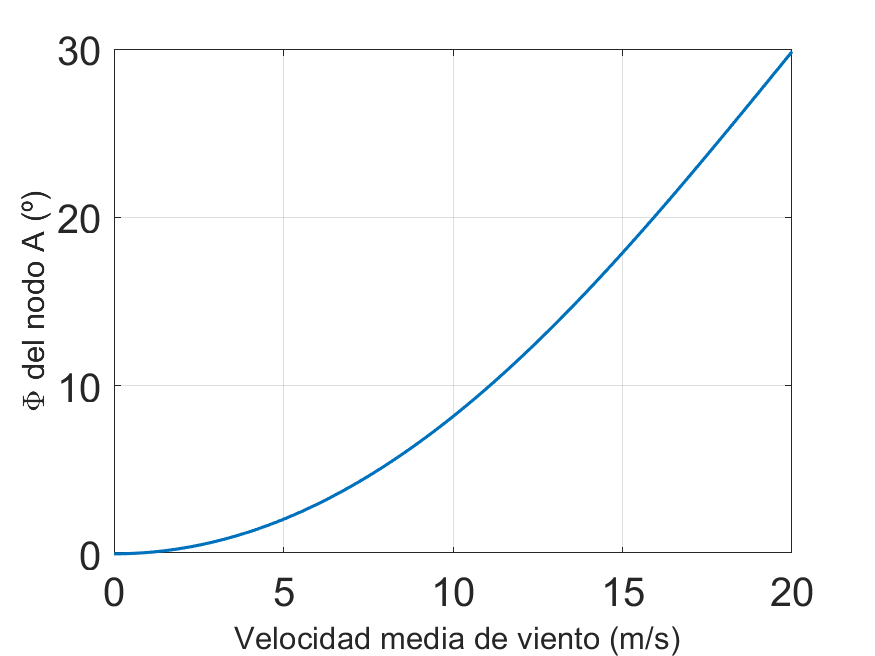
\includegraphics[width=80mm]{./imagenes/ResultadosNumericos/SimpleCable/Angulo_Foti.png}
	\caption{Ángulo de balanceo $\Phi$ en función de la velocidad media $W(t)$.}
	\label{fig:CableAngulo}
\end{figure}

El ejemplo permite inferir que la respuesta numérica del modelo representa de manera acorde y aceptable las dinámicas del fenómeno para conductores de transmisión eléctrica bajo ciertas hipótesis. Dada la semejanza en los resultados arrojados por la formulación, respecto a la bibliografía estudiada, es posible aventurarse a la aplicación de casos más complejos. 



\section{Sistema de transmisión eléctrica }\label{Sec:RN:TransmissionSystem}
Este ejemplo ataca el objetivo central de este trabajo: modelar sistemas de transmisión eléctricas afectados por vientos extremos no sinópticos, en particular, TC. Las estructuras de suministro en alta tensión constan de un tendido eléctrico anclado mediante torres, las que sostienen el conductor garantizando un traslado de la corriente de manera segura y confiable. El dominio del ejemplo consta de tres torres equiespaciadas colocadas consecutivamente y dos vanos de idéntico largo $D_v= 206.5$ m tal cual se indica el Esquema \ref{fig:Transmission:EsquemaGeneral}.  Para el conductor de control se etiquetan los puntos de fijación $\text{A}$ y $\text{D}$ a la torre 1 y 2, respectivamente. También, se identifican los nodos en el punto medio del primer y segundo vano con los literales $\text{C}$ y $\text{B}$, respectivamente. Con el objetivo de representar una geometría real de una línea de alta tensión y no aborrecer al lector con descripciones de propiedades, los conductores de la simulación se corresponden con el ejemplo resuelto de la Sección \ref{Sec:RN:FotiCable} y cuyas propiedades mecánicas se explicitan en la Tabla \ref{table:RN:FotiCable:propiedadesCable}.  


\begin{figure}[htbp]
	\centering
	\def\svgwidth{120mm}
	\input{./imagenes/ResultadosNumericos/TransmissionTormenta/IlustracionTormenta.pdf_tex}
	\caption{Esquema del sistema de transmisión.}
	\label{fig:Transmission:EsquemaGeneral}
\end{figure}

En Uruguay los tendidos eléctricos de alta tensión son aquellos que transportan un voltaje mayor a $72.5$ kV. Este valor de tensión es eminentemente peligroso y para asegurar que la torre se encuentre aterrada se utilizan elementos aisladores. Para el modelar las cadenas se utilizaron elementos de barras tipo Green presentados en \citep{Crisfield}. Además, se consideró un módulo de elasticidad aproximado $E = 70$ GPa según los estudios experimentales realizados por  \cite{MoralesAisladores}.


Al igual que los aisladores, las barras de las torres metálicas se modelaron con elementos de Green, con una ley material Saint-Venant-Kirchhoff con $E= 300$ GPa y $\nu=0.3$. Su geometría fue suministrada por el Ingeniero Agustín Téliz, cuya tesis de maestría consiste en el modelado y optimizado estructural de las mismas.  Estos valores se corresponden con un acero ASTM A 572 laminado en caliente, usual en este tipo de estructuras, junto al A36 y ASTM º65. Estas torres tienen una altura máxima de $44$ m y un ancho entre los opuestos de la cercha de $14.8$ m. Además, estas son capaces de soportar 6 lineas,  a cada altura sostienen cada una de las fases eléctricas. Las líneas se encuentran colocadas a tres cotas distintas $L_1=$ 31.75 $m$, $L_2=$ 26.03 $m$, $L_3=$ 39.76 $m$, tal y como se muestra en \ref{fig:RN:Transmission:Torre}. 

\begin{figure}[h]
	\centering
	\def\svgwidth{80mm}
	\input{./imagenes/ResultadosNumericos/TransmissionTormenta/IlusTorre.pdf_tex}
	\caption{Esquema geométrico de cotas principales en la torre. }
	\label{fig:RN:Transmission:Torre}
\end{figure}

La simulación se separa en dos etapas, primeramente partiendo de la configuración solución al problema estático del peso propio, se aplica la gravedad según el eje $-z$ tal cual se muestra en la Figura \ref{fig:Transmission:EsquemaGeneral}. Nuevamente, al igual que en el Ejemplo \ref{Sec:RN:FotiCable} , esto suprime posibles inestabilidades cuando las tensiones son próximas a cero. Esta etapa tomó 100 segundos y es estabilizada por el amortiguamiento. Este se calculó según lo descrito en la Sección \ref{Sec:MET:HipotesisModeladoNumerico} resultando $c=\rho_a C_d dc l_{elem} \overline{v}=0.15$ Ns/m.

Posteriormente se aplica una fuerza correspondiente a un perfil de tormenta convectiva capturado en la referencia \citep{stengel2017measurements}, positiva según el eje $x$. No se tienen en cuenta fluctuaciones espaciales siendo la velocidad una componente uniforme. Es menester destacar que la tormenta convectiva se aplicó únicamente al vano que sitúa entre la torre 1 y 2, con el objetivo de extraer resultados respecto al comportamiento flexional en el plano $yz$, lo que se evidenciará a continuación la diferencia de las trayectorias entre los nodos $\text{A}$, $\text{C}$, $\text{D}$ y $\text{B}$. La aplicación de la tormenta en una fracción del dominio se basa en que estos fenómenos tienen dimensiones espaciales del orden de 40 metros a 40 kilómetros según \cite{fujita1985downburst}, consecuentemente es factible que la tormenta afecte a una fracción del tendido. Los valores de fuerza y velocidad asociadas a la coordenada $x$ entre los nodos A y D para cada instante se muestran a continuación:

\begingroup
\begin{figure}[htbp]
	\centering
	\subfigure[Carga aplicada sobre los nodos. ]{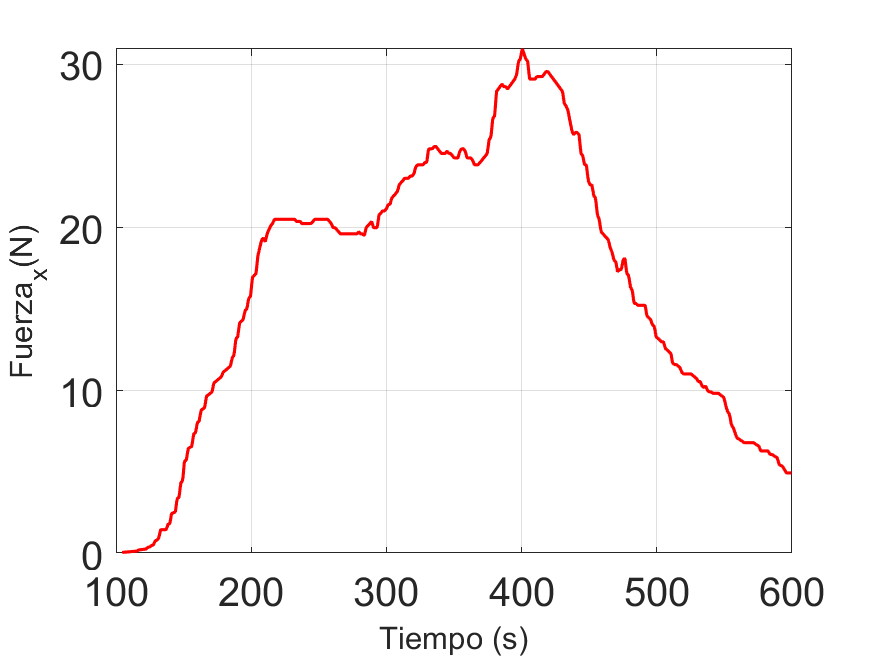
\includegraphics[width=0.48\textwidth]{./imagenes/ResultadosNumericos/TransmissionTormenta/FuerzaNodalX_TS.png}\label{fig:RN:Transmission:FuerzaTormentaX}}
	\subfigure[Perfil de velocidades de viento.] {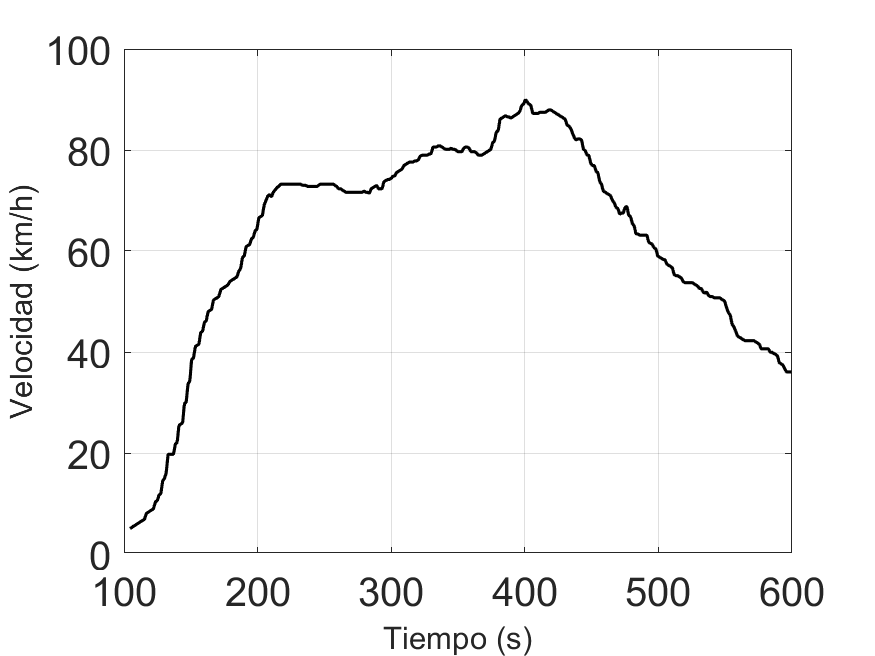
\includegraphics[width=0.48\textwidth]{./imagenes/ResultadosNumericos/TransmissionTormenta/VelocidadNodalX_TS.png}\label{fig:RN:Transmission:VelocidadTormentaX}}	
	\label{fig:RN:Transmission:ForceVelTormenta}
\end{figure}
\endgroup

%Las tormentas severas generan CD donde las velocidades aumentan vertiginosamente en pequeños intervalos de tiempo, alcanzando umbrales de hasta 270 km/h \cite{fujita1985downburst}. Para este modelo, el perfil representado es de menor tenor, mas no el aumento súbito del fenómeno. La velocidad se eleva del valor nulo a 80 km/h en menos de 3 minutos, tal y como se observa en la Figura \ref{fig:RN:Transmission:VelocidadTormentaX}. Debido al impacto de del viento sobre el conductor se generan fuerzas, estas se calcularon con los valores de coeficiente drag y fórmula detalladas en el Ejemplo \ref{Sec:RN:FotiCable} anterior extraídos de la referencia \cite{Foti2016}.

Se compararon cuantitativamente las oscilaciones entre fases (A-A', X-X', Z-Z') de la Figura \ref{fig:RN:Transmission:Torre}, no apreciándose sensibles diferencias, tanto en desplazamientos lineales como angulares. Por otra parte, no existen apreciables variaciones a ambos lados del plano transversal de simetría (entre A-A'). Esto se explica debido a la distribución espejada de la geometría y el hecho de omitir las variaciones en el flujo de aire aguas abajo del cable que recibe antes el impacto del flujo. Aclarados los aspectos mencionados, y considerando que los desplazamientos de la torre aumentan con la cota, se eligió el nodo \textit{A} como variable de control. Para este nodo se registraron su desplazamiento en los ejes $x$ y $z$ como también el ángulo de oscilación \gls{AnguloEj3} tal y cual se observa en la Figura \ref{fig:RN:Transmission:Angulo}.

\begin{figure}[htbp]
	\centering
	\def\svgwidth{80mm}
	\input{./imagenes/ResultadosNumericos/TransmissionTormenta/IlustracionAngulo.pdf_tex}
	\caption{Ilustración de magnitudes de balanceo.}
	\label{fig:RN:Transmission:Angulo}
\end{figure}

El modelado numérico del ejemplo se realizó considerando 200 elementos de viga corrotacional por conductor, utilizando un paso temporal de $\Delta T =0.5$ s y un algoritmo de resolución numérica HHT con un parámetro característico $\alpha=-0.05$, luego de un procedimiento iterativo de ajuste de parámetros se realizaron las simulaciones en un período 30 hs aproximado con tolerancias en desplazamientos y en fuerzas residuales de $10^{-5}$ m y 10$^{-5}$ N, respectivamente.

A continuación se muestran los desplazamientos verticales y horizontales de los extremo libre de las cadenas aisladoras, nominadas con las letras $\text{A}$, $\text{D}$. En estos se observa un comportamiento inercial y una relación entre el perfil de fuerza y desplazamientos. Este comportamiento homólogo entre ambas magnitudes externas, responde a un argumento basado en el análisis en frecuencia del sistema, donde la función de transferencia desfasa a ambas magnitudes en estado estacionario. En \ref{fig:RN:Transmission:DispXAD} y \ref{fig:RN:Transmission:DispZAD} se observan los desplazamientos en vertical y transversal, respectivamente. En ambas figuras es posible notar que debido a la intensidad del viento sobre los conductores entre la torre 1 y 2, el nodo $\text{A}$ desarrolla un movimiento de mayor amplitud. No obstante, cabe destacar el carácter sintético de las condiciones de borde para el nodo ya que el modelo no representa las cargas inerciales de los vanos contiguos a este. 


\begingroup
\centering
\begin{figure}[htbp]
	\centering
	\subfigure[Desplazamientos en $x$ nodos \text{A}, \text{D}. ]{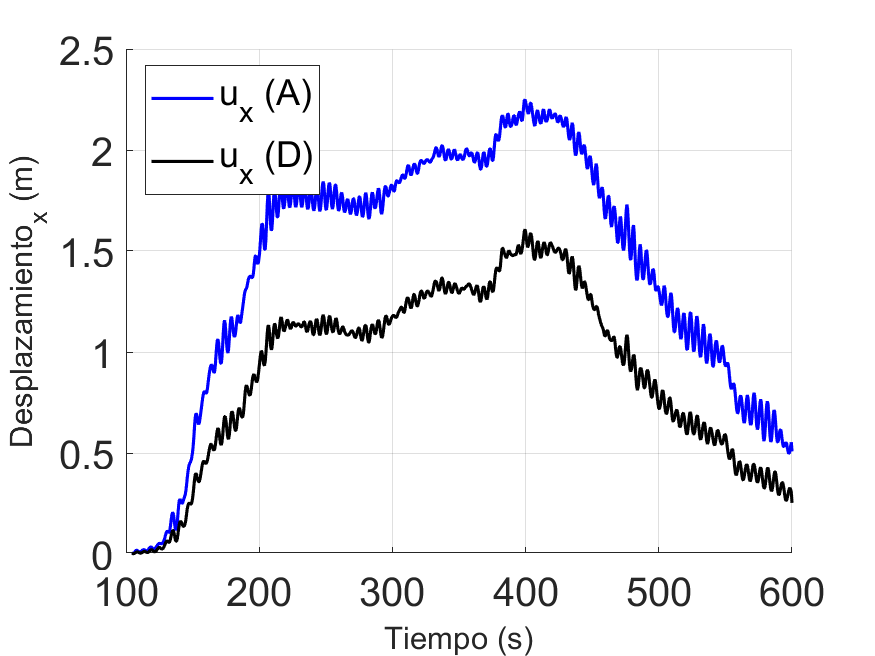
\includegraphics[width=0.48\textwidth]{./imagenes/ResultadosNumericos/TransmissionTormenta/DispXTS_NodeAD.png}\label{fig:RN:Transmission:DispXAD}}
	\subfigure[Desplazamientos en $z$ nodo \text{A}, \text{D}.] {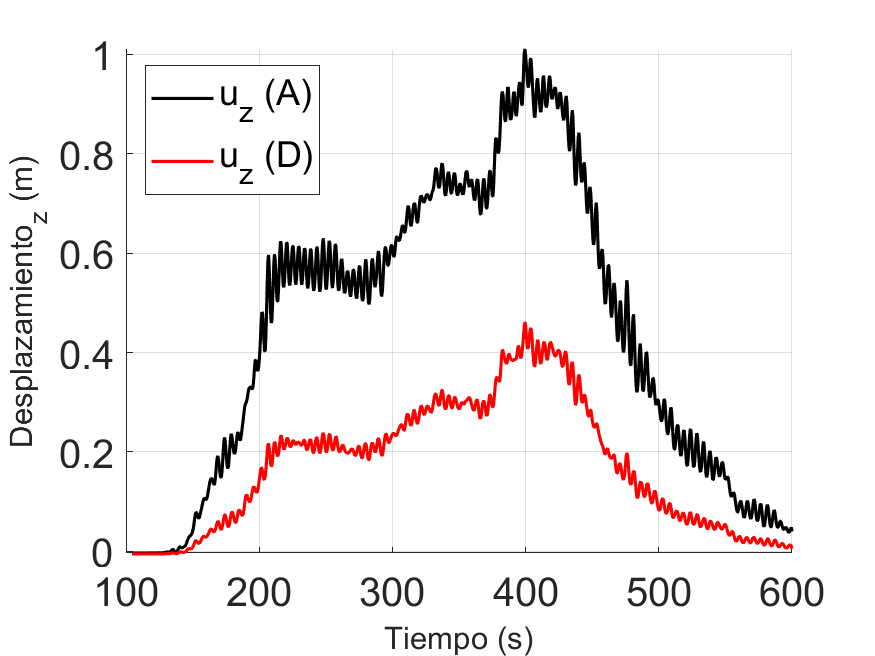
\includegraphics[width=0.48\textwidth]{./imagenes/ResultadosNumericos/TransmissionTormenta/DispZTS_NodeAD.png}\label{fig:RN:Transmission:DispZAD}}
	\caption{Desplazamientos de las cadenas aisladoras \text{A} y \text{D}.} \label{fig:RN:Transmission:DispsAD}
\end{figure}
\endgroup

Además de los elementos aisladores, los puntos medios en el vano del conductor también despliegan grandes desplazamientos, este fenómeno resulta indeseable debido a múltiples factores, entre ellos: las restricciones de seguridad sobre movimientos máximos, las inductancias magnéticas que puedan generar voltajes peligrosos a objetos paramagnéticos circundantes, y la proximidad entre fases que puede devenir en cortocircuito y daño sobre los componentes. Por estas razones, en las Figuras \ref{fig:RN:Transmission:DispsCB} se ilustran los desplazamientos para los nodos $\text{B}$ y $\text{C}$. 


\begingroup
\centering
\begin{figure}[htbp]
	\centering
	\subfigure[Desplazamientos en $x$ nodos B y C. ]{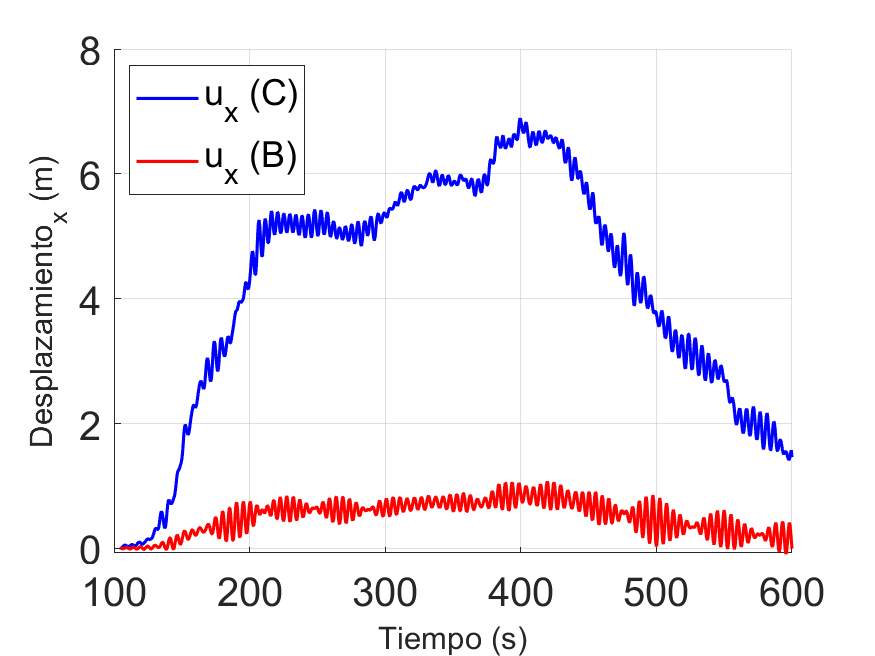
\includegraphics[width=0.48\textwidth]{./imagenes/ResultadosNumericos/TransmissionTormenta/DispXTS_NodeCB.png}\label{fig:RN:Transmission:DispXCB}}
	\subfigure[Desplazamientos en $z$ nodo B y C.] {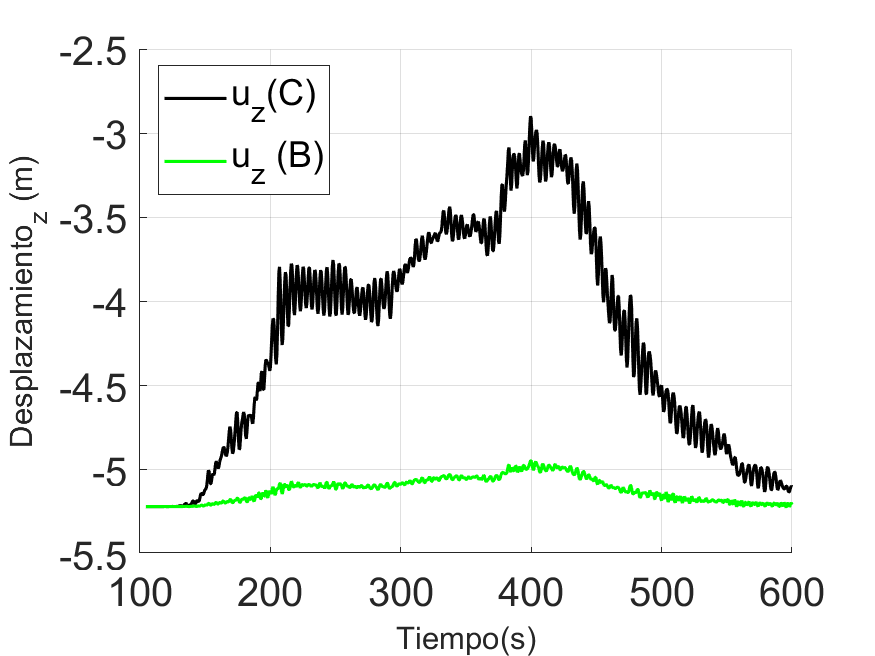
\includegraphics[width=0.48\textwidth]{./imagenes/ResultadosNumericos/TransmissionTormenta/DispZTS_NodeCB.png}\label{fig:RN:Transmission:DispZCB}}
	\caption{Desplazamientos de los nodos medios B y C. \label{fig:RN:Transmission:DispsCB}}
\end{figure}
\endgroup

En la Figura \ref{fig:RN:Transmission:DispXCB} se aprecia que el orden de los movimientos, para ambos nodos, es menor $8$ m durante el dominio temporal. Como la separación entre estos es de unos 14 metros lo que garantiza que no habrá impactos entre conductores, aun sin considerar desplazamientos sincrónicos entre ambas líneas. No obstante, otras arquitecturas de torres poseen un conductor central, para este caso las posibilidades de choque son mayores y la amenaza debe considerarse a la hora del diseño. En la Figura \ref{fig:RN:Transmission:DispZCB} se muestra que el descenso máximo de la línea se presenta en la primer etapa de simulación, alcanzando un valor de $5.2$ m. Esto resulta evidente y trivial dado el sentido de la fuerza ejercida por el viento, pero es una magnitud relevante de seguridad al momento de la instalación, para regular la fuerza de pre-tensado. Al igual que en el par de Figuras \ref{fig:RN:Transmission:DispsAD}, en \ref{fig:RN:Transmission:DispsCB} se aprecian comportamientos morfológicos semejantes en las historias de desplazamiento entre nodos. Cabe notar que, a pesar de que los perfiles son análogos entre los distintos puntos, los desplazamientos en puntos medios representados en las Figuras \ref{fig:RN:Transmission:DispsCB} presentan una mayor fluctuación temporal respecto los de las cadenas aisladoras mostradas en las Figuras \ref{fig:RN:Transmission:DispsAD}.

Por otra parte, en las Figuras \ref{fig:RN:Transmission:DispsCB} se observan indicios de inestabilidades numéricas, debido a altas frecuencias inducidas por el método computacional o modos de resonancia.

En virtud de escudriñar la relación entre los perfiles de fuerza y las variables cinemáticas se elaboró la Figura \ref{fig:RN:Trnamission:CurvaCargaDisp} carga desplazamiento para el nodo A. En abscisas, se colocó el valor del ángulo de balanceo, y en ordenadas la fuerza nodal originada por la tormenta. Además de plasmar los resultados numéricos se graficó un cálculo estático ampliamente utilizado en la bibliografía, sobre todo en el área de ingeniería del viento \citep{stengel2017measurements}, \citep{duranona2009analysis} \citep{yang2016nonlinear}.


\begin{figure}[htbp]
	\centering
	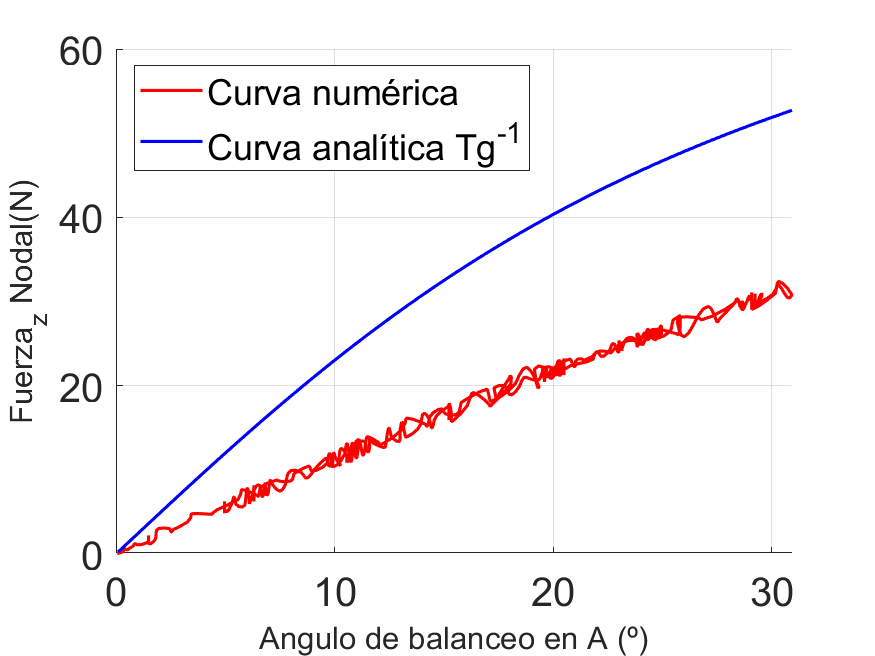
\includegraphics[width=100mm]{./imagenes/ResultadosNumericos/TransmissionTormenta/FuerzaAngulo_TS.png}
	\caption{Curva analítica y numérica carga desplazamiento.}
	\label{fig:RN:Trnamission:CurvaCargaDisp}
\end{figure}

El cálculo analítico resulta de un planteo estático plano, donde se iguala la tangente del ángulo con el cociente entre la fuerza total ejercida sobre el conductor y su peso. Este razonamiento no tiene en cuenta las componentes inerciales, tanto de la cadena aisladora como también del conductor, cuyas aceleraciones pueden afectar las fuerzas internas trasmitidas al elemento aislador. Asimismo, ese cálculo desprecia la componente 3D del movimiento en la coordenada axial, proveniente de las distintas orientaciones de la línea respecto al ángulo de incidencia del flujo. En la Figura \ref{fig:RN:Trnamission:CurvaCargaDisp} se evidencian las diferencias entre los modelos y como el cálculo analítico arroja valores sobredimensionados, respecto al umbral de velocidad que produciría el impacto, según los resultados del modelo implementado. Con el objetivo de ilustrar visualmente sobre las deformaciones de la estructura y las fluctuaciones axiales mencionadas, se muestran la configuración indeformadas en gris y las deformadas con una barra de colores en desplazamientos para el instante $t=400 s$ en la Figura \ref{fig:RN:Transmission:Deformadas}.


\begin{figure}[htbp]
	\centering
	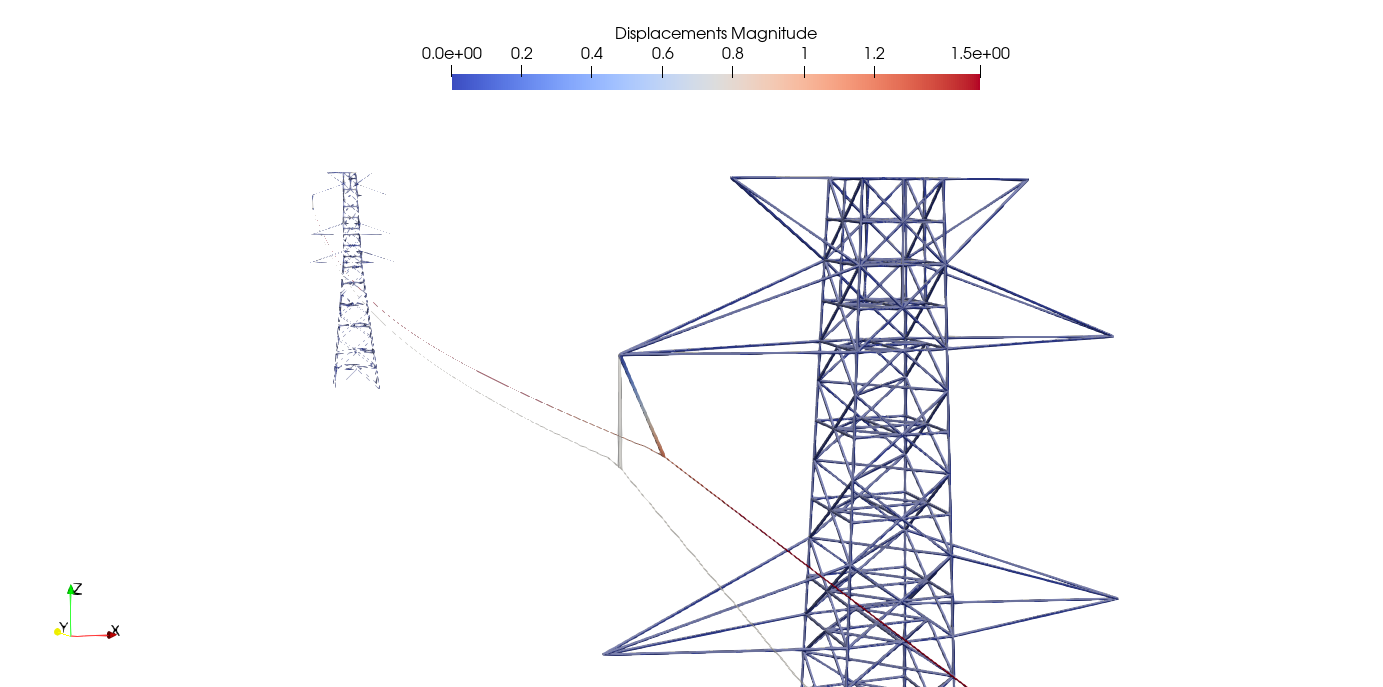
\includegraphics[width=120mm]{./imagenes/ResultadosNumericos/TransmissionTormenta/Deformadas.png}
	\caption{Estructura indeformada y deformada para $t=400$ s.}
	\label{fig:RN:Transmission:Deformadas}
\end{figure} 
